\documentclass[conference]{IEEEtran}
\IEEEoverridecommandlockouts
% The preceding line is only needed to identify funding in the first footnote. If that is unneeded, please comment it out.
\usepackage{cite}
\usepackage{amsmath,amssymb,amsfonts}
\usepackage{algorithmic}
\usepackage{graphicx}
\usepackage{textcomp}
\usepackage{xcolor}
\usepackage{color}
\usepackage{listings}
\usepackage{float}
\usepackage[hidelinks]{hyperref}
\def\BibTeX{{\rm B\kern-.05em{\sc i\kern-.025em b}\kern-.08em
    T\kern-.1667em\lower.7ex\hbox{E}\kern-.125emX}}
\begin{document}

\definecolor{dkgreen}{rgb}{0,0.6,0}
\definecolor{gray}{rgb}{0.5,0.5,0.5}
\definecolor{mauve}{rgb}{0.58,0,0.82}

\lstset{frame=single,
    language=[sharp]C,
    aboveskip=3mm,
    belowskip=3mm,
    showstringspaces=false,
    columns=flexible,
    basicstyle={\scriptsize\ttfamily},
    numbers=none,
    numberstyle=\tiny\color{gray},
    keywordstyle=\color{blue},
    commentstyle=\color{dkgreen},
    stringstyle=\color{mauve},
    breaklines=true,
    breakatwhitespace=true,
    tabsize=3
}


\title{Supervisory Control and Data Acquisition on an air-heating process \\
{\footnotesize}
}

\author{\IEEEauthorblockN{Ruben Vander Elst}
\IEEEauthorblockA{\textit{University of South-Eastern Norway (Campus Porsgrunn)} \\
Porsgrunn, Norway}
}

\maketitle


\begin{abstract}
This paper describes a SCADA system for the control, monitoring and data acquisition of an air heating process. The system incorporates ideas from concepts such as Hardware-in-the-loop. Source Code is made available for the complete system.
\end{abstract}

\begin{IEEEkeywords}
SCADA, HIL, Database, Control Systems, USN
\end{IEEEkeywords}

\section{Introduction}
Supervisory Control and Data Acquisition systems(SCADA) are systems that control, monitor and collect data from process plants and machines. The architecture typically consists of network communication, Human Machine Interfaces (HMI) and computers\cite{wikipediacontributors_2022_scada}.

The aim of a SCADA system is to provide high-level supervision and control of processes. Although SCADA has existed since the 1960s\cite{yang_2019_ict}, modern technology makes it more available, cost-effective and useful. The availability and insight to SCADA technology is limited since such systems are often developed for larger industrial appliances, and the intellectual property then belongs to commercial actors. However, open source, free or low-cost components needed to establish a SCADA architecture are highly available on the internet today. This paper proposes a complete SCADA system and provides the necessary code to build the system.

The system proposed in this paper is designed for the control and monitoring of an air-heating process. This process and some requirements for the SCADA system has been provided by the University of South-Eastern Norway (USN). A system diagram is depicted in Figure \ref{system_diagram}

\begin{figure}[H]
    \centering
    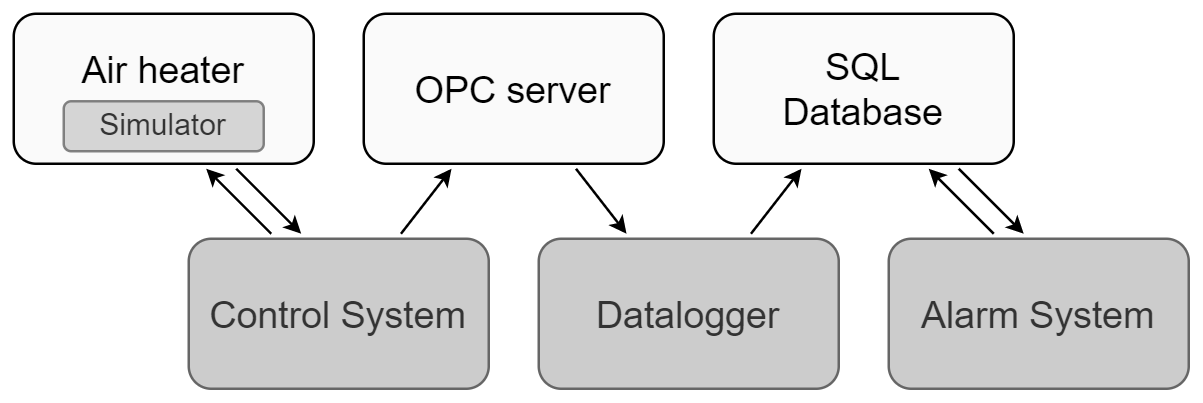
\includegraphics[scale=0.18]{media/system_diagram_bw.png}
    \caption{A system diagram showing the logical components of the proposed SCADA system}
    \label{system_diagram}
\end{figure}

\section{Method}
\subsection{The air-heating process}
The process was examined to secure a firm understanding of its requirements and operational purpose. The air-heating process is a small scale air heater, consisting of a pipe system with manually controlled fans on both the inlet and outlet. The inlet has a heater medium that can be controlled by analog input (0-5V) and thereby heat the incoming air. A temperature sensor is mounted on the outlet of the pipe system, where its value (1-5V) can be measured by external devices. To be able to interface to this process, a USB DAQ device from National Instruments is used (NI-DAQ-6008). This makes it possible to control and monitor the process through computers. Figure \ref{air_heater} shows a picture of the process.

\begin{figure}[H]
    \centering
    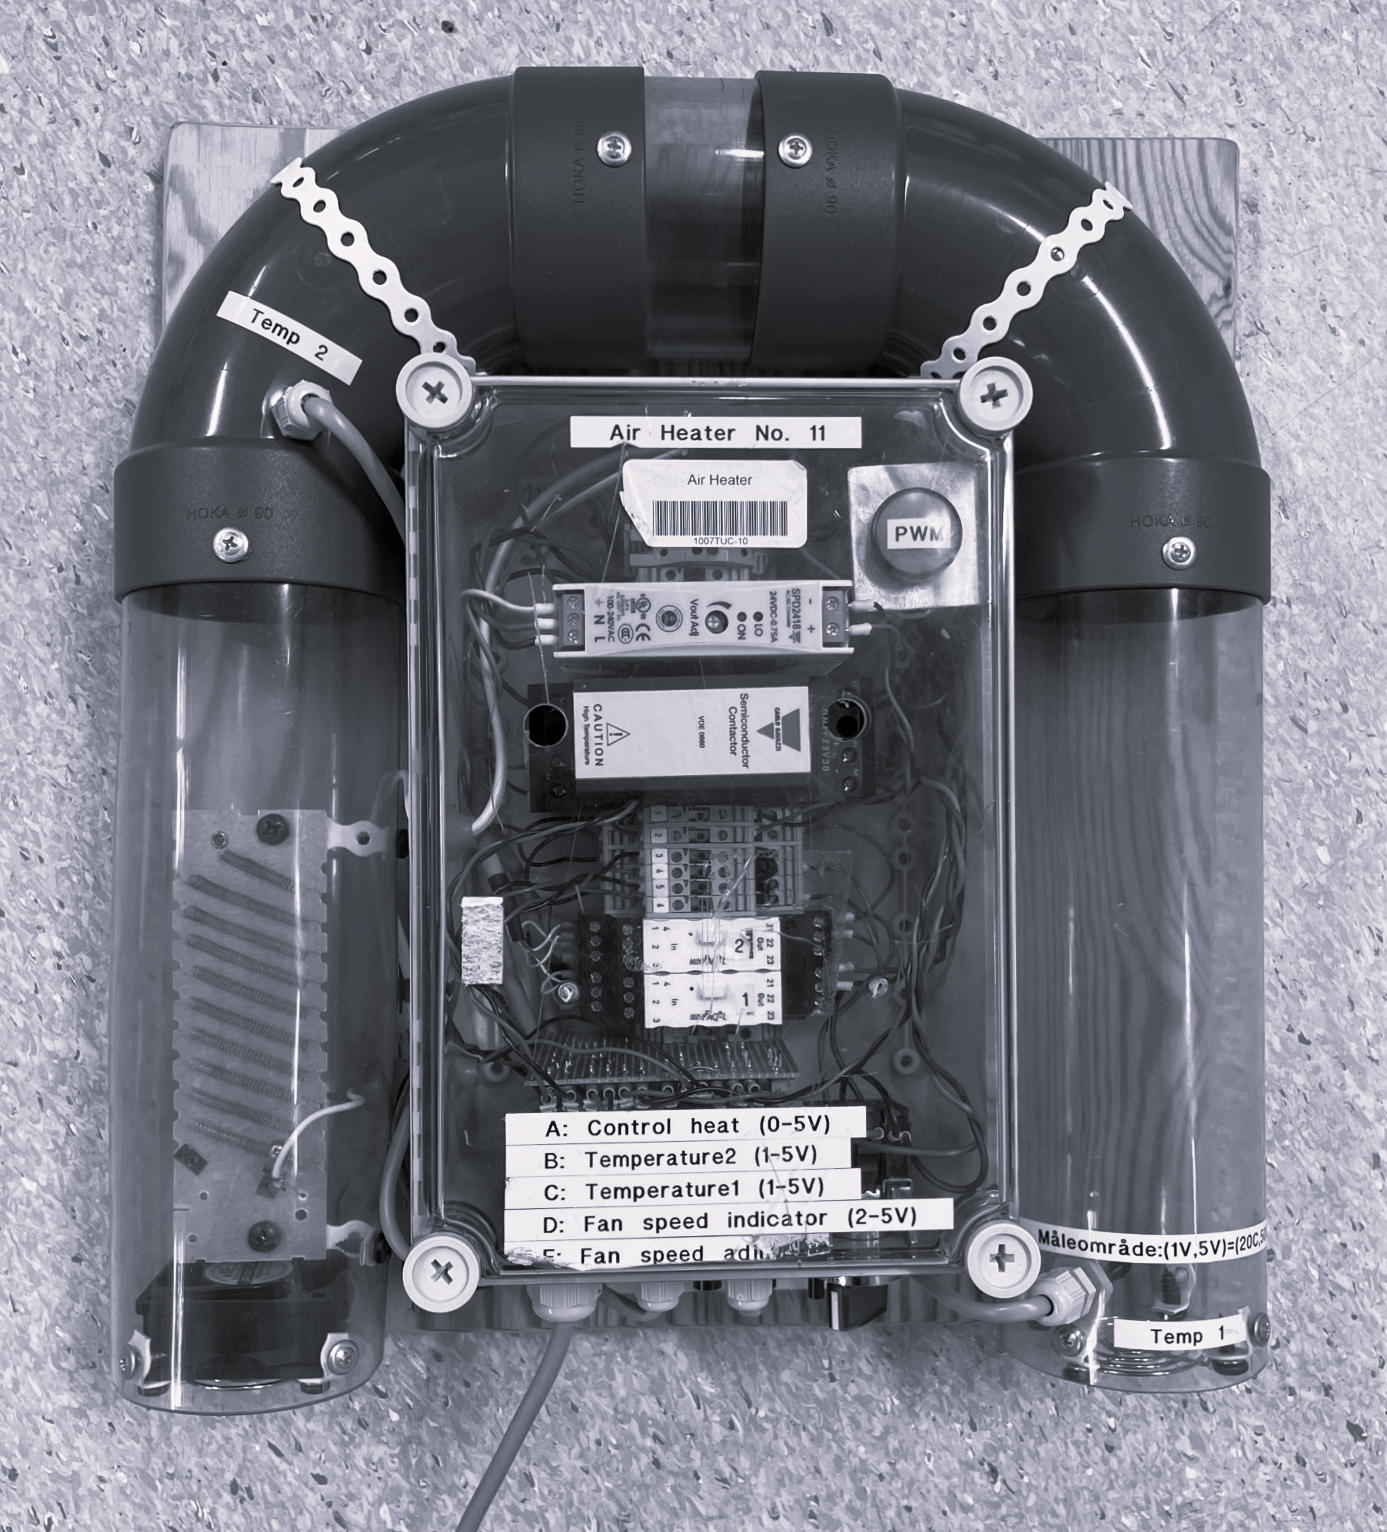
\includegraphics[scale=0.13]{media/air_heater.png}
    \caption{A picture of the air-heating process provided bu USN}
    \label{air_heater}
\end{figure}

A mathematical model of the air-heating process has been provided by USN (Equation \ref{air_heat_model}). This model can be implemented in a simulator and hence serve as a digital twin for the physical process.

\begin{equation}
    \label{air_heat_model}
    \dot{T}_{out} = \frac{1}{\theta_t}\left(-T_{out}+\left(K_h u (t-\theta_d)+T_{env} \right)\right)
\end{equation}

Where:
\begin{itemize}
    \item[] $\dot{T}_{out}$ is the temperature derivative, describing the temperature rate of change in celsius per seconds,
    \item[] $T_{out}$ is the temperature in degrees celsius measured at the outlet of the heater,
    \item[] $u$ is the control signal in the range of 1-5 volts,
    \item[] $\theta_s$ is the time constant in seconds,
    \item[] $K_h$ is the heater gain in degrees celsius per volt,
    \item[] $\theta_d$ is the time delay in seconds, describing the transport time of air within the heating process,
    \item[] $T_{env}$ is the environmental temperature in degrees celsius,
    \item[] $t$ is the real-time point of the measurements.
\end{itemize}

Since the SCADA system is comprised of computers, a time-discrete model is necessary. The Forward Euler method, has characteristics that is suitable for this application. This method replaces $\dot{T}_{out}$ as such:
\begin{equation}
    \label{t_out_discrete}
    \dot{T}_{out} = \frac{T_{out1} - T_{out}}{T_s}
\end{equation}

Where $T_s$ is the sampling time. Applying equation (\ref{t_out_discrete}) to the original model (\ref{air_heat_model}) gives the discrete version shown in equation (\ref{air_heat_model_discrete}).

\begin{equation}
    \label{air_heat_model_discrete}
    T_{out1} = \frac{T_{out} + T_s\left(-T_{out} + \left(K_h u_d[i] + T_{env}\right)\right)}{\theta_t}
\end{equation}

Where $u_d[i]$ is the time-delayed control signal, replacing the expression $u(t-\theta_d)$. At this point, the mathematical model is possible to implemented in computer code.

\subsection{PI Controller}
A discrete linear quadratic optimal controller with integral action has been published \cite{ruscio_2012_discrete}. This controller is suitable for the air-heating process, as it is expressed on a time-discrete form, and has properties that resembles a PI controller. The two main equations for this controller is shown in (\ref{ruscio_pi}) and (\ref{ruscio_pi_z}). 

\begin{equation}
    \label{ruscio_pi}
    u_k = K_p (r - y) + \frac{K_p}{T_i}z
\end{equation}
\begin{equation}
    \label{ruscio_pi_z}
    z = z + T_s (r - y)
\end{equation}

Where:
\begin{itemize}
    \item[] $u_k$ is the controller gain,
    \item[] $K_p$ is the proportional parameter,
    \item[] $r$ is the setpoint reference,
    \item[] $y$ is the process value,
    \item[] $T_i$ is the integral parameter,
    \item[] $T_s$ is the sampling time,
    \item[] $z$ is the incremental variable that affects the integral time.
\end{itemize}

This can be implemented in computer code. However, helping mechanisms is necessary in code to limit $u_k$ in the required range. This is necessary because the physical process and DAQ device only accept a signal between 0-5 Volts. In addition, the heater medium has a limitation that is not represented in linear models such as equation \ref{ruscio_pi} and equation \ref{ruscio_pi_z}. This limitation is called saturation and can cause the integration time to accumulate endlessly. A way to handle saturation is called anti-windup and is typically achieved by limiting the integration time within a range that corresponds to the physical process. This has been handled in the proposed system by limiting the incrementation of $z$.

\subsection{Low-pass filter}
Filters are used in digital signal processing to reduce unwanted noise in physical appliances. Noise can easily affect operation and cause the controller to misinterpret signals from the process. A low-pass filter can be expressed with equation (\ref{filter_eq_a}) and (\ref{filter_eq}).
\begin{equation}
    \label{filter_eq_a}
    a = \frac{T_s}{T_s + T_f}
\end{equation}
\begin{equation}
    \label{filter_eq}
    y_{f+1} = (1 - a) y_{f} + a y
\end{equation}

Where:
\begin{itemize}
    \item[] $T_s$ is the sampling time,
    \item[] $T_f$ is the period time,
    \item[] $y_{f+1}$ is the next filtered value,
    \item[] $y_{f}$ is the previous filtered value,
    \item[] $y$ is the input value to be filtered.
\end{itemize}

The values chosen for $T_s$ and $T_f$ determines the cutoff frequency of the low-pass filter. For example, if $T_f \lim \rightarrow 0$ the cutoff frequency is approaching $\infty$. In a low-pass filter, this means that there is no filtering of the signal, and the filter is in principal only forwarding whatever it receives. This was used in the development process by setting $T_f$ to a very low value, and subsequently adjusting it until satisfactory results could be observed on the process and control signals.

\subsection{System Requirements}
Specific system requirements has been provided by USN:
\begin{itemize}
    \item A Database should be designed using erwin Data Modeler software
    \item The Database should be implement using SQL Server
    \item The Control System should be implemented in C\# and send data to an OPC Server from the air-heating 
    \item A PI(D) controller and low-pass filter should be implemented in C\#
    \item The Control system should write data to an OPC server
    \item The system should incorporate a Datalogging System, written in C\# that logs data from the OPC server to the SQL Database
    \item The system should incorporate an Alarm Generation and Monitoring System, written in C\#.
    \item The different subsystems should be implemented as separate Applications because they should be able to 
    run on different computers in a network (distributed).
    \item Describe relevant Cyber Security issues with the system
\end{itemize} 

These requirements, together with the process examination was used to establish a high-level system diagram (Figure \ref{system_diagram}) and develop the necessary components. The source code can be accessed in this shared folder:
\url{https://www.icloud.com/iclouddrive/06ehn_bpO0iF-w1zSBHoIGWnA#SCADA}

\section{Results}
\subsection{Control System}

The Control system was implemented in C\#, Windows Forms, with a user interface for tuning of the PI controller, toggling between simulation or real process, and for the plotting of process data onto charts. A screenshot of the user interface is shown in Figure \ref{control_system}. The user interface has three charts that show Process Value (Temperature), Setpoint, Control Value and the internal variable $z$. The interface also supports adjustments of the PI controllers parameters $K_p$ and $T_i$ as well as the desired setpoint. A start and stop button is provided, and the possibility to toggle between simulation and real process. Finally, two numerical indicators shows the real time value of the control and process signals. 

\begin{figure}[H]
    \centering
    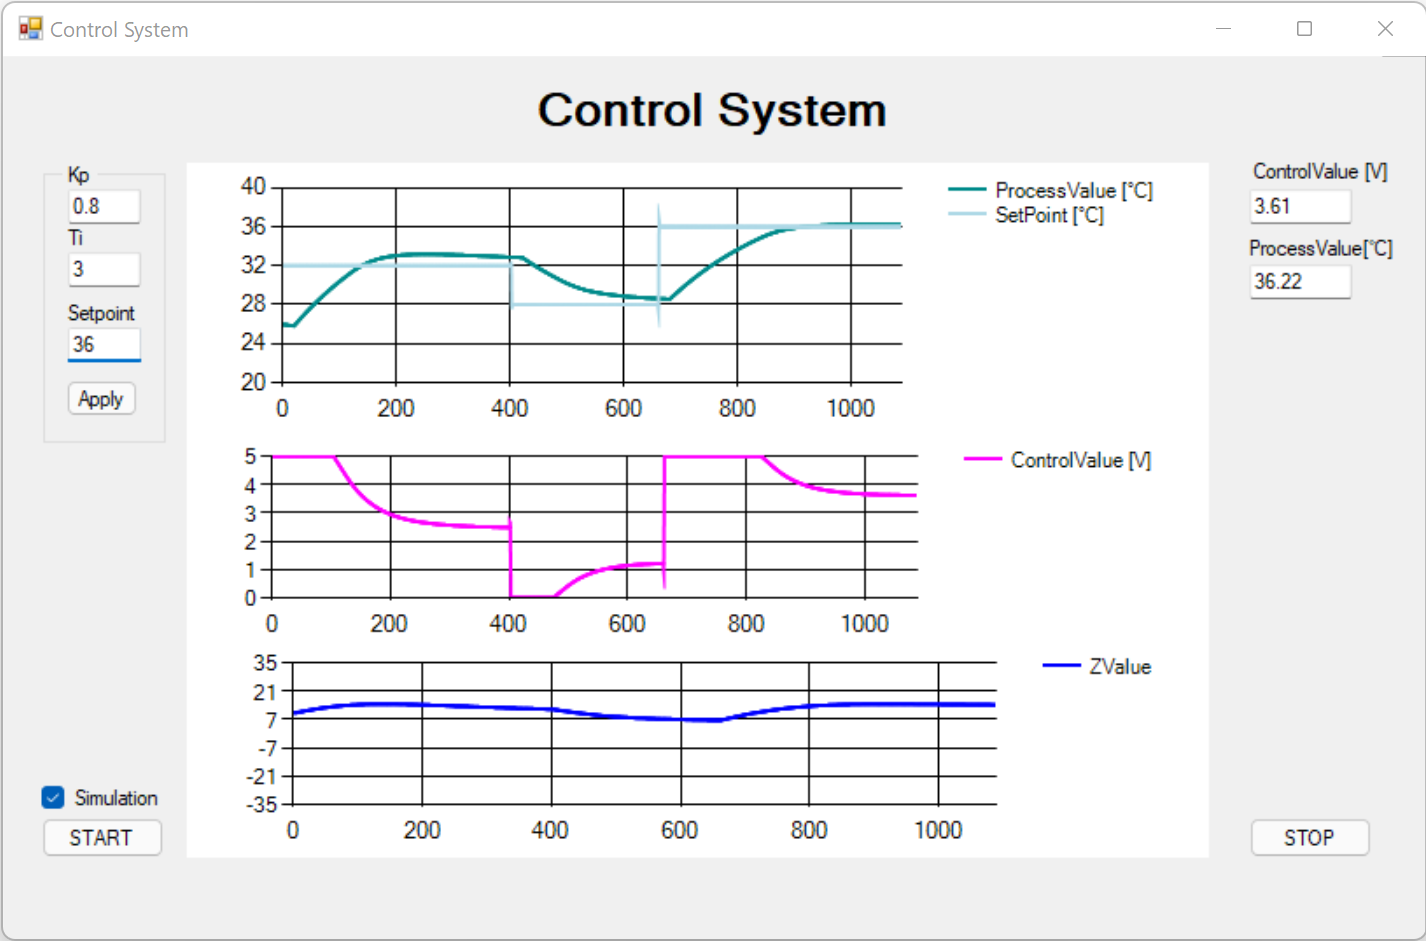
\includegraphics[scale=0.38]{media/control_system.png}
    \caption{The user interface for the control system, showing the process' response to setpoint changes and calculated control signal. }
    \label{control_system}    
\end{figure}

\subsubsection{PI Controller}
The PI Controller was implemented in C\# using Equation (\ref{ruscio_pi}) and (\ref{ruscio_pi_z}). The controller was tuned with parameters shown in Table \ref{pid_params}. The method used to find these parameters was to utilize the benefit of the simulator and experiment until the process could achieve fast control with acceptable stability.

\begin{table}[H]
    \centering
    \begin{tabular}{ |l|c| }
        \hline
        Parameter & Value \\ 
        \hline \hline
        $K_p$ & 0.8\\
        $T_i$ & 3 [s] \\
        $T_s$ & 0.1 [s]\\
        \hline
    \end{tabular}
    \vspace{5pt}
    \caption{Parameters obtained from testing the PI controller against the simulated and real process}
    \label{pid_params}
\end{table}

To implement anti-windup, the necessary limitations for $z$ was found by attempting to match the natural saturation of the heater medium. The range was determined to be $-5<z<20$. The necessity and performance of this limitation is shown in Figure \ref{anti_windup4}.

\begin{figure}[H]
    \centering
    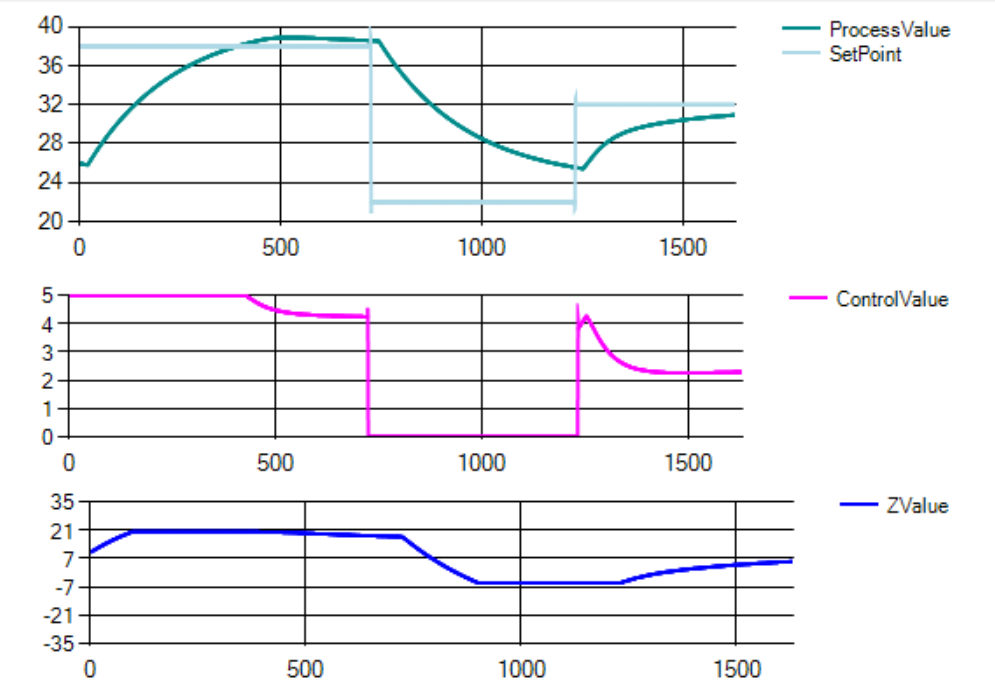
\includegraphics[scale=0.3]{media/anti_windup4.png}
    \caption{Anti-windup through limitation of $z$, ensuring that the saturation of the heater gain medium is handled by the PI controller}
    \label{anti_windup4}
\end{figure}

The main method for the PI controller with limitations on $u_k$ and $z$ is shown in listing \ref{pi_controller_code}.

\begin{lstlisting}[caption={Implementation of the PI controller in C\#}, label={pi_controller_code}]
public double Control(double y)
{
    // Main calculations
    double uk;
    double e = r - y;
    uk = Kp * e + (Kp / Ti) * z;
    z += T_s * e;

    // Limit uk between 0 and 5 (volts)
    if (uk > 5)
    {
        uk = 5;
    }
    else if (uk < 0)
    {
        uk = 0;
    }

    // Anti windup for z
    if (z > 20)
    {
        z = 20;
    }
    else if (z < -5)
    {
        z = -5;
    }


    return uk;
}
\end{lstlisting}

\subsubsection{Air-heater simulator}
The air-heating simulator was implemented in C\# by using equation (\ref{air_heat_model_discrete}). To accomplish the correct time-delay of the controller gain $u_d[i]$ an array was created. Since the sampling time is set 0.1 seconds, an array with a length of 20 could be used to generate a delay of 2 seconds. This gave satisfactory results. The model was controlled by the PI controller with three setpoint changes (30-35-40$^{\circ}$C) and compared to the same setpoint changes when controlling the physical process. The control results are shown in Figure \ref{sim_vs_real} where the simulator is used the first 1100ms and the physical process the remaining time. The simulator showed clear resemblance to the physical process. The setpoint changes was repeated to evaluate and tune the model parameters, resulting in the values shown in Table \ref{air_heat_model_params}. 

\begin{figure}[H]
    \centering
    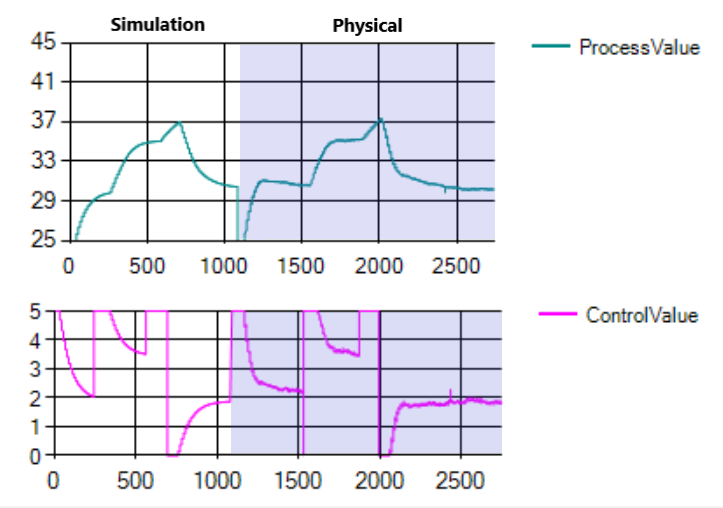
\includegraphics[scale=0.4]{media/sim_vs_real.png}
    \caption{Chart plots of multiple setpoint changes on the simulator vs the physical process}
    \label{sim_vs_real}
\end{figure}

\begin{table}[H]
    \centering
    \begin{tabular}{ |l|c| }
        \hline
        Parameter & Value \\ 
        \hline \hline
        $K_h$ & 3.35 [C/V]\\
        $T_{env}$ & 24 [C]\\
        $\theta_d$ & 2 [s]\\
        $\theta_t$ & 22 [s]\\
        \hline
    \end{tabular}
    \vspace{5pt}
    \caption{Parameters obtained from testing the process simulator against the real process}
    \label{air_heat_model_params}
\end{table}

\subsubsection{Filter}
The filter was implemented by using Equation (\ref{filter_eq_a}) and (\ref{filter_eq}). Through trial and error, filter parameters was found. These are provided in Table \ref{filter_params}. The result showed a substantial improvement in the control signal. This can be seen by comparing the physical part of Figure \ref{sim_vs_real} with the following Figure (Figure \ref{anti_windup_cut})

\begin{figure}[H]
    \centering
    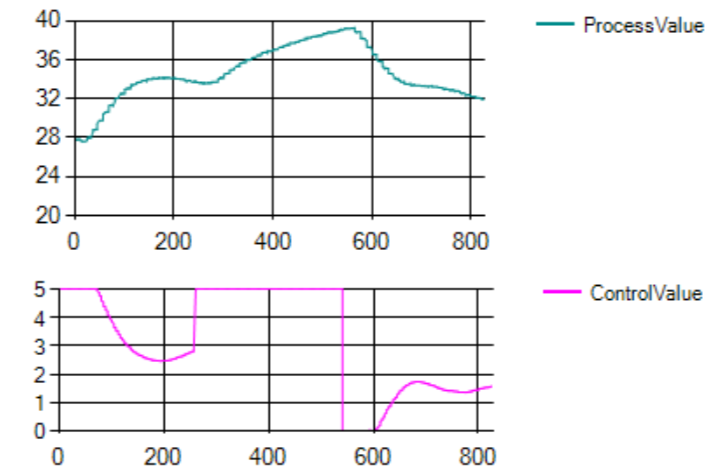
\includegraphics[scale=0.8]{media/anti_windup_cut.png}
    \caption{Testing the low-pass filter on the physical process. Compared to figure \ref{sim_vs_real}, the reduction of noise is substantial.}
    \label{anti_windup_cut}
\end{figure}

\begin{table}[H]
    \centering
    \begin{tabular}{ |l|c| }
        \hline
        Parameter & Value \\ 
        \hline \hline
        $T_s$ & 0.01 [s]\\
        $T_f$ & 0.2 [s]\\
        \hline
    \end{tabular}
    \vspace{5pt}
    \caption{Parameters obtained from testing the filter against the real process}
    \label{filter_params}
\end{table}

\subsection{OPC UA Server}
The OPC UA server was integrated using the free OPC server from Integration Objects. The Server was configured as of Table \ref{opc_address_space}, with the tags intended for exchange between applications, and their correct data type. These tags could then be configured in the code for both the Control System and the Datalogger.

\begin{table}[H]
    \centering
    \begin{tabular}{ |l|l|l|l| }
        \hline
        Tag Name & Data Type & AccessRights & Simulated \\ 
        \hline \hline
        PV & IO\_Double & RW & FALSE \\ \hline
        SP & IO\_Double & RW & FALSE \\ \hline
        u & IO\_Double & RW & FALSE \\ \hline
        Kp & IO\_Double & RW & FALSE \\ \hline
        Ti & IO\_Double & RW & FALSE \\ \hline
        d & IO\_Double & RW & FALSE \\ \hline
        z & IO\_Double & RW & FALSE \\ \hline
\end{tabular}
\vspace{5pt}
\caption{Content of configuration file "AddressSpace.csv" for the OPC UA server}
\label{opc_address_space}
\end{table}

\subsection{Datalogger}
The datalogger was implemented in C\# and configured with the OPC tags described in Table \ref{opc_address_space}. Some charts where added to make sure the data received from the OPC server was correct. A screenshot of this application is shown in Figure \ref{datalogger}. Upon reading the values from the OPC server and plotting some of them to charts, the datalogger sends this data to the SQL server using a stored procedure.

\begin{figure}[H]
    \centering
    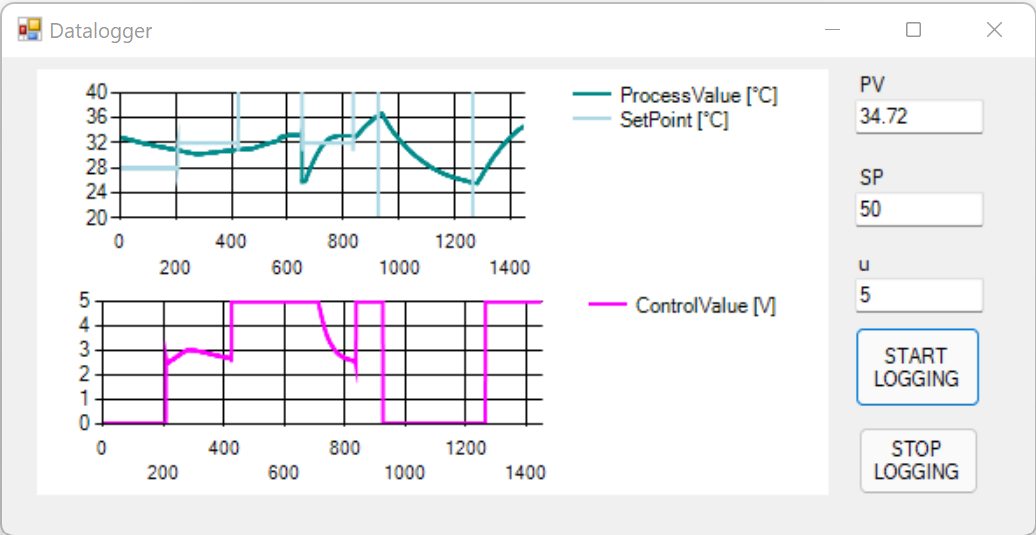
\includegraphics[scale=0.55]{media/datalogger2.png}
    \caption{User interface for the Datalogger application}
    \label{datalogger}    
\end{figure}

\subsection{SQL Database}
The SQL Database was designed using the ERwin data modeler software. Principles affecting the design choices was modularity, scalability and history. Modularity; to easily adapt the database design when needed. Scalability; to ensure that the database can handle the addition of tags, alarms, and functionality. History; to provide storage for large and valuable datasets.

The data that is stored is key to monitor and troubleshoot the process. Although outside of the scope of the proposed SCADA system, big data sets collected from the process can lay the foundation for advancements like system identification, model predictive control or machine learning. In addition, big data sets can be very valuable for the evaluation of the process and is at the core of some of the benefits of SCADA and the concept of data acquisition.

These considerations resulted in the design of three tables, TAG, ALARM and HISTORY, as seen in Figure \ref{erwin_diagram}. The TAG table is used to add tags like "Process Value" or "Setpoint" and values can be written to these tags live. This design allows for scalability, as any number of tags can be added. The HISTORY table "subscribes" to the TAG table by collecting every value written to the tags and assigning it a date stamp, the tag ID and a quality status. This shows the history principle, that much data can safely be stored in this table, and crucial info like date, tag ID and quality is kept. The ALARM table monitors the TAG and HISTORY tables to determine alarms and warnings. This shows the modularity of the design, that the alarms can be generated both by the HISTORY or the TAG table.

\begin{figure}[H]
    \centering
    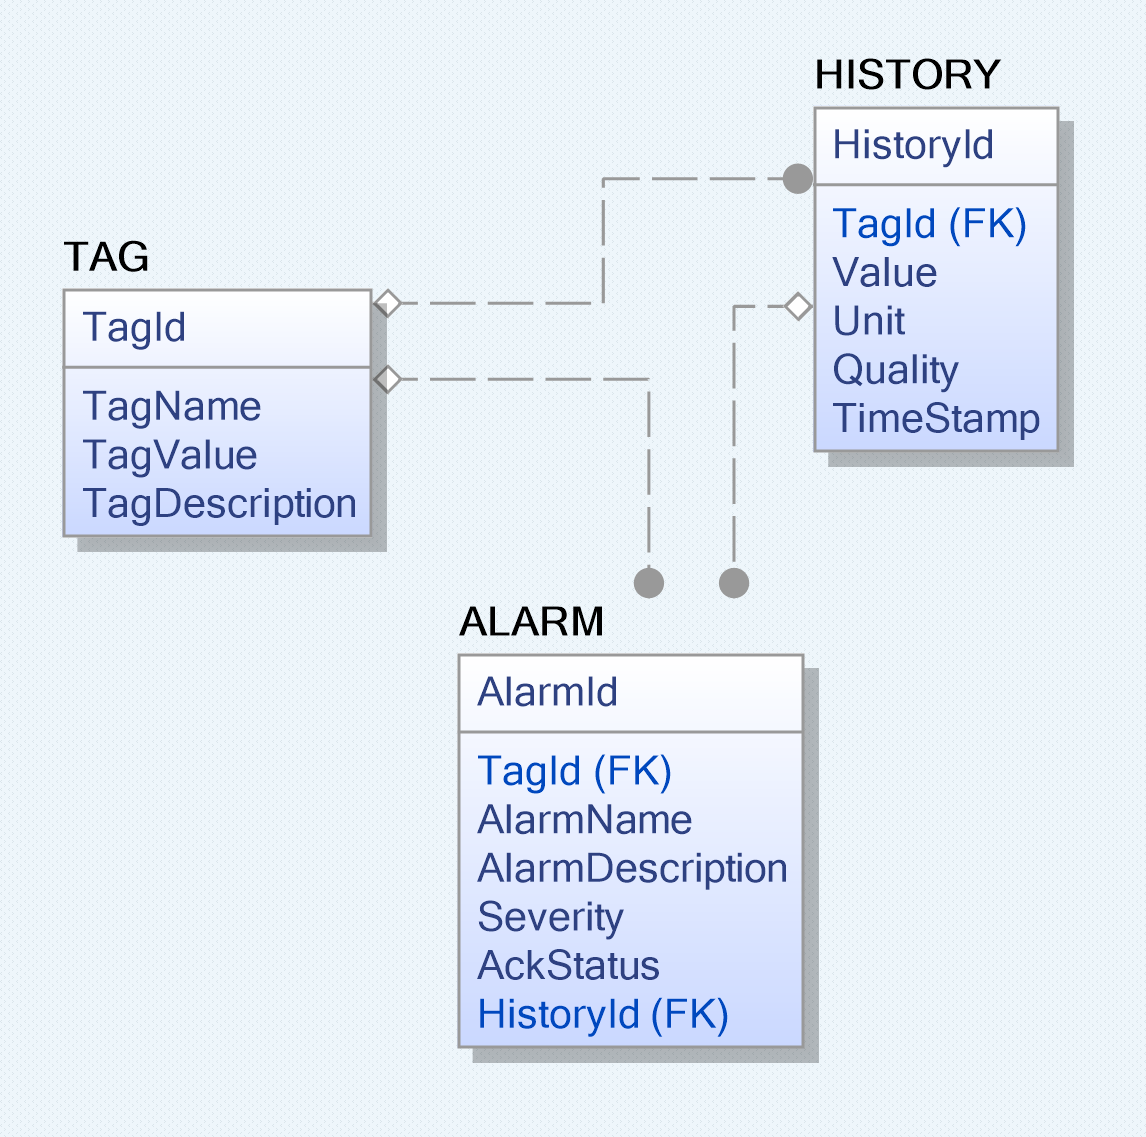
\includegraphics[scale=0.4]{media/erwin_diagram.png}
    \caption{ERwin diagram showing the database design}
    \label{erwin_diagram}
\end{figure}

Stored procedures was written to sanitize incoming queries. This ensures that the database is not vulnerable to SQL injections. Procedures were also made for the ability to acknowledge alarms and to configure tags. A separate SQL script was made for the configuration of the tags, to enable either easy access for technical users of the system, or for future integration into applications. This script is shown in listing \ref{configure_tags}.

\begin{lstlisting}[caption={ConfigureTags.sql}, label={configure_tags},language=SQL]
EXEC ConfigureTag @TagId = 1, @TagName = 'PV', @TagDescription = 'Temperature measured on the outlet of the Process';
EXEC ConfigureTag @TagId = 2, @TagName = 'SP', @TagDescription = 'Set point for the desired Temperature';
EXEC ConfigureTag @TagId = 3, @TagName = 'u', @TagDescription = 'Control value sent to the Air Heater';
EXEC ConfigureTag @TagId = 4, @TagName = 'Ti', @TagDescription = 'Controller Integral parameter';
EXEC ConfigureTag @TagId = 5, @TagName = 'Kp', @TagDescription = 'Controller Proportional parameter';
EXEC ConfigureTag @TagId = 6, @TagName = 'd', @TagDescription = 'Controller Derivative parameter';
EXEC ConfigureTag @TagId = 7, @TagName = 'z', @TagDescription = 'Variable for integral calculation';
\end{lstlisting}

\subsection{Alarm System}
An alarm system was implemented in C\#. This system reads the alarms generated from the database and displays them with color codes matching the severity of the alarm. The user can browse alarms and acknowledge alarms individually. Upon acknowledging an alarm, the alarm system uses a stored procedure to store the acknowledgement in the database. A screenshot of the user interface is shown in Figure \ref{alarm_system}

\begin{figure}[H]
    \centering
    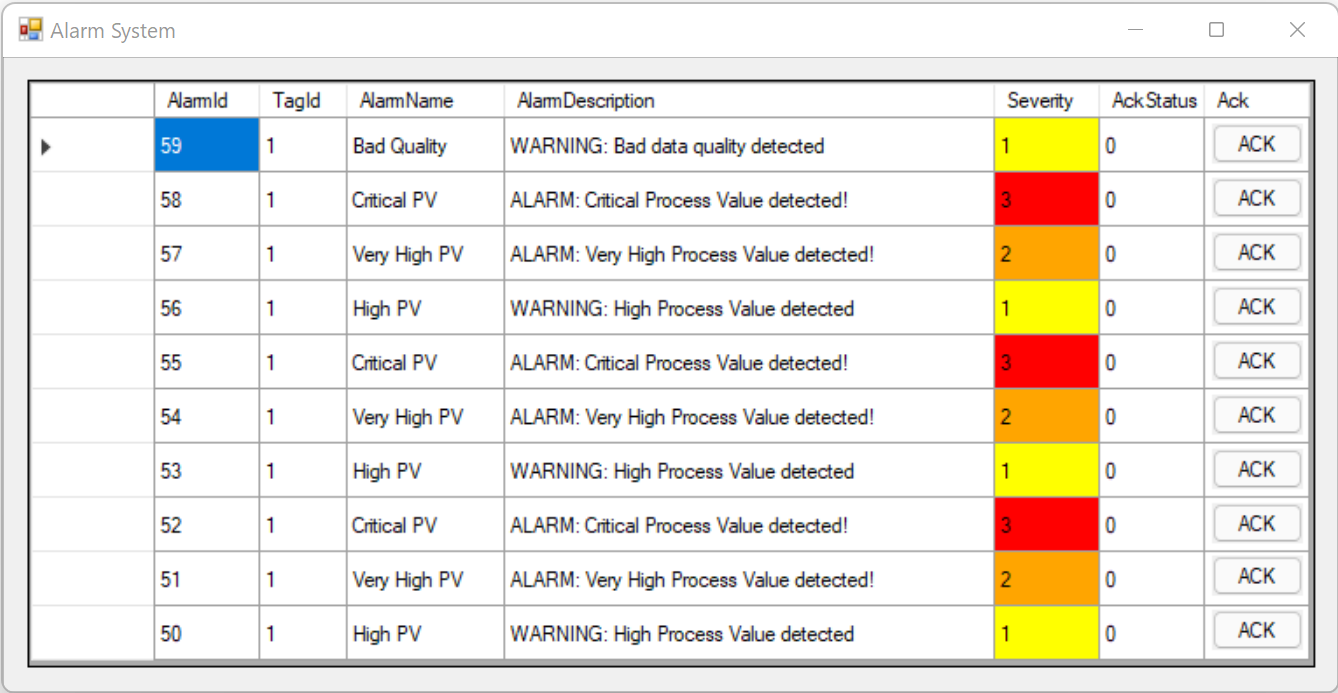
\includegraphics[scale=0.42]{media/alarm_system.png}
    \caption{The user interface for the alarm system}
    \label{alarm_system}
\end{figure}

\section{Discussion}
The proposed system demonstrates a fully functional SCADA system and satisfy the necessary requirements. However, the system may benefit from certain improvements. Some of which will be discussed in this section.

\subsection{Control System}
The control system manages to control the process with a decent speed and acceptable stability. However, certain improvements should be considered. In the filtered example, in Figure \ref{anti_windup_cut}, small "steps" in the process value can be observed. This is not noise, but related to the implementation of DAQ communication. In the C\# implementation, a new "Task" and an analog in/out channel is created before reading/writing data to the DAQ device every 0.1 seconds. This increases the time used to read and write data to the process. When examining Figure \ref{anti_windup_cut}, this phenomenon can only be observed on the process value. This is because the plotted values for the control signal is a value calculated internally \textit{before} communicating with the DAQ device. Plotting the control signal on the output of the DAQ device should show the same "steps" as observed in the process value chart, if the assumed cause is true.  Regardless of this, the PI controller calculated correct values for the control signal.

The tuning method used to find $K_p$ and $T_i$ parameters for the controller is trial and error. This can be done in a more sophisticated way, by for example using the Skogestad method. However, some tuning methods like the Ziegler \& Nichols is not possible as the heating medium in the process is not powerful enough to bring the system into a marginally stable condition.

\subsection{Database and use of data}
The current configuration of the Database designed for the SCADA system does not delete any entries. This means that the size of the database will increase endlessly. In a production environment, this should be taken into consideration by implementing clean-up policies or providing sufficient storage space.

The current data that are stored in the database are mainly process data and acknowledgement statuses. However, more operational data can be beneficial to add, for example user actions from the control system or connection details to the OPC server.

\subsection{Alarm system}
For production use, the alarm system might benefit from the addition of a user login and tracking integration. This would allow the acknowledgements of alarms to be tied to a user. Another improvement that would be beneficial is the addition of more Alarms and warnings, such as bad connections to the OPC server, unnatural process behavior or wrong user inputs.

Finally, a more comprehensive notification solution for the alarms should be considered such as email, sms, interfacing to physical horns or lamps etc. This can be done based on the criticality of the alarms and process in operation.

\subsection{Cyber Security}
Effort have been done to limit the vulnerabilities in the proposed SCADA system. However, since the system is heavily based on the windows platform, it will share the same vulnerabilities as the Windows operating system. It is therefore important to harden the operating system by closing unused ports, disabling unwanted software (de-bloating) and removing or restricting the systems access to the internet. Since the solution provided is software based, the hardware that is used to run the software will be an important factor in the limitation of the systems attack surface. For example, computers should have "USB-Guarding" to avoid vulnerability to the insertion of unwanted media. USB and LAN has been typical ways to attack systems disconnected from the internet, like the famous case of the Stuxnet virus \cite{mims_2017}, which is a very relevant cyber security incident affecting a control system with a SCADA-like solution in a nuclear facility in Iran.

Besides the physical and digital infrastructure the system is installed on, the system itself has not been built with validation mechanisms on data exchange between the sub systems. Another service (like a malicious program) could for example send data to the OPC server and in that way inject data into the database, causing the alarm generations to either malfunction or generate false alarms. This vulnerability could also be exploited to preform a Denial of Service (DOS) attack by flooding the OPC server with information so that the correct information from the control system is lost.

Moreover, the SQL database uses a traditional username-password authentication that has limited security, especially since the login information is stored in clear text in the configuration files for the connecting services. A malicious actor can simply access these files and use the login credentials to send custom SQL queries to the database. To prevent this vulnerability from being exploited, the C\# programs can be compiled to binary applications, hiding the credentials to the database, and the Database can be configured with minimal permissions to the user in question, should the credentials get astray. 

Finally, the systems hardware should incorporate firewalls between networks that are not related to the SCADA. Anti-virus and monitoring services should also be installed on the computers used for the system, to be able to detect, investigate and respond to a cyber security incident.

\subsection{Redundancy}
The proposed system is not designed with redundancy. This means that the system, with its current configuration, has multiple single-points of failure, and would not be suitable for safety critical operation. However, upgrading the system to support redundancy is possible, and can be a valuable consideration for future development.


\section{Conclusion}
The proposed system demonstrates that the availability and cost effectiveness of SCADA are very good with todays technology. Many valuable features has been tied to gether to a fully functioning system with minimal cost and short development time. The proposed system can be modified and deployed to many applications, though the physical and digital infrastructure that is used for the system is crucial for the security of the system.

\bibliographystyle{IEEEtran}
\bibliography{IEEEabrv,SCADA.bib}

\end{document}
